%%%%%%%%%%%%%%%%%%%%%%%%%%%%%%%%%%%%%%%%%
% Masters/Doctoral Thesis 
% LaTeX Template
% Version 2.5 (27/8/17)
%
% This template was downloaded from:
% http://www.LaTeXTemplates.com
%
% Version 2.x major modifications by:
% Vel (vel@latextemplates.com)
%
% This template is based on a template by:
% Steve Gunn (http://users.ecs.soton.ac.uk/srg/softwaretools/document/templates/)
% Sunil Patel (http://www.sunilpatel.co.uk/thesis-template/)
%
% Template license:
% CC BY-NC-SA 3.0 (http://creativecommons.org/licenses/by-nc-sa/3.0/)
%
%%%%%%%%%%%%%%%%%%%%%%%%%%%%%%%%%%%%%%%%%

%----------------------------------------------------------------------------------------
%	PACKAGES AND OTHER DOCUMENT CONFIGURATIONS
%----------------------------------------------------------------------------------------

\documentclass[
11pt, % The default document font size, options: 10pt, 11pt, 12pt
oneside, % Two side (alternating margins) for binding by default, uncomment to switch to one side
english, % ngerman for German
% singlespacing, % Single line spacing, alternatives: onehalfspacing or doublespacing
% TODO - something is overrulling our doublespacing, need to find out what
onehalfspacing,
%draft, % Uncomment to enable draft mode (no pictures, no links, overfull hboxes indicated)
%nolistspacing, % If the document is onehalfspacing or doublespacing, uncomment this to set spacing in lists to single
%liststotoc, % Uncomment to add the list of figures/tables/etc to the table of contents
%toctotoc, % Uncomment to add the main table of contents to the table of contents
%parskip, % Uncomment to add space between paragraphs
%nohyperref, % Uncomment to not load the hyperref package
headsepline, % Uncomment to get a line under the header
%chapterinoneline, % Uncomment to place the chapter title next to the number on one line
consistentlayout, % Uncomment to change the layout of the declaration, abstract and acknowledgements pages to match the default layout
reqno, % align equation numbers to right
]{MastersDoctoralThesis} % The class file specifying the document structure

% This goes with setspace package
% \onehalfspacing

\usepackage[utf8]{inputenc} % Required for inputting international characters
\usepackage[T1]{fontenc} % Output font encoding for international characters
% Allow exact placement of images
\usepackage{float} 

\usepackage{mathpazo} % Use the Palatino font by default - Lara Chammas used this one
% Looks time TNR so let's go with that
% \usepackage{newtxmath,newtxtext} % Times New Roman - the required type
% filler to get idea of formatting
\usepackage{lipsum}
% pdf pages for appending original project proposal
\usepackage{pdfpages}

\usepackage[backend=bibtex,style=authoryear,natbib=true]{biblatex} % Use the bibtex backend with the authoryear citation style (which resembles APA)

\addbibresource{dissertation.bib} % The filename of the bibliography

\usepackage[autostyle=true]{csquotes} % Required to generate language-dependent quotes in the bibliography
\usepackage{listings} % Add this line to include the listings package, and render algorithms
\usepackage{mathtools} % for floor symbol
%----------------------------------------------------------------------------------------
%	MARGIN SETTINGS
%----------------------------------------------------------------------------------------

\geometry{
	paper=a4paper, % Change to letterpaper for US letter
	inner=2.5cm, % Inner margin
	outer=2.5cm, % Outer margin
	% bindingoffset=.5cm, % Binding offset
	top=1.5cm, % Top margin
	bottom=1.5cm, % Bottom margin
	%showframe, % Uncomment to show how the type block is set on the page
}

%----------------------------------------------------------------------------------------
%	THESIS INFORMATION
%----------------------------------------------------------------------------------------

\thesistitle{Evaluation of autonomous vehicles \\ using Artificial Neural Networks in \\ complex traffic systems} % Your thesis title, this is used in the title and abstract, print it elsewhere with \ttitle
\supervisor{Artur Garcez} % Your supervisor's name, this is used in the title page, print it elsewhere with \supname
\examiner{} % Your examiner's name, this is not currently used anywhere in the template, print it elsewhere with \examname
\degree{Doctor of Philosophy} % Your degree name, this is used in the title page and abstract, print it elsewhere with \degreename
\author{Daniel Sikar} % Your name, this is used in the title page and abstract, print it elsewhere with \authorname
\addresses{} % Your address, this is not currently used anywhere in the template, print it elsewhere with \addressname

\subject{Biological Sciences} % Your subject area, this is not currently used anywhere in the template, print it elsewhere with \subjectname
\keywords{Autonomous Vehicles, Convolutional Neural Networks} % Keywords for your thesis, this is not currently used anywhere in the template, print it elsewhere with \keywordnames
\university{City, University of London} % Your university's name and URL, this is used in the title page and abstract, print it elsewhere with \univname
\department{\href{http://department.university.com}{Department or School Name}} % Your department's name and URL, this is used in the title page and abstract, print it elsewhere with \deptname
\group{\href{http://researchgroup.university.com}{Research Group Name}} % Your research group's name and URL, this is used in the title page, print it elsewhere with \groupname
\faculty{\href{http://faculty.university.com}{Faculty Name}} % Your faculty's name and URL, this is used in the title page and abstract, print it elsewhere with \facname

\AtBeginDocument{
\hypersetup{pdftitle=\ttitle} % Set the PDF's title to your title
\hypersetup{pdfauthor=\authorname} % Set the PDF's author to your name
\hypersetup{pdfkeywords=\keywordnames} % Set the PDF's keywords to your keywords
\hypersetup{hidelinks}
}

% do not indent paragraphs
\setlength\parindent{0pt}
% Add 
\setlength{\parskip}{0.5em} % changes vertical space between paragraphs, alternatively use pt unit e.g. {10pt} %
% Appendix
\usepackage{appendix}

\begin{document}

\frontmatter % Use roman page numbering style (i, ii, iii, iv...) for the pre-content pages

\pagestyle{plain} % Default to the plain heading style until the thesis style is called for the body content

%----------------------------------------------------------------------------------------
%	TITLE PAGE
%----------------------------------------------------------------------------------------

\begin{titlepage}
\begin{center}

\vspace*{.06\textheight}
{\scshape\LARGE \univname\par}\vspace{1.5cm} % University name
\textsc{\Large PhD thesis}\\[0.5cm] % Thesis type
\textsc{\Large Project Report}\\[0.5cm]
\textsc{\Large 2024}\\[0.5cm]

\HRule \\[0.4cm] % Horizontal line
{\huge \bfseries \ttitle\par}\vspace{0.4cm} % Thesis title
\HRule \\[3.5cm] % Horizontal line
 
% \begin{minipage}[t]{0.4\textwidth}
\begin{flushleft} \large
% \emph{Author:}\\
\authorname \\ [1cm]
%\href{http://www.johnsmith.com}{\authorname} % Author name - remove the \href bracket to remove the link
% \end{flushleft}
% \end{minipage}
% \begin{minipage}[t]{0.4\textwidth}
% \begin{flushright} \large

\emph{Supervised by:} 
\supname \\ [3.5cm] % Supervisor name - remove the \href bracket to remove the link  
\end{flushleft}
% \end{flushright}
%\end{minipage}\\[3cm]
 

%\large \textit{A thesis submitted in fulfillment of the requirements\\ for the degree of %\degreename}\\[0.3cm] % University requirement text
%\textit{in the}\\[0.4cm]
%\groupname\\\deptname\\[2cm] % Research group name and department name
 

{\large \today}\\[4cm] % Date
%\includegraphics{Logo} % University/department logo - uncomment to place it
 
%vfill
\end{center}
\end{titlepage}

%----------------------------------------------------------------------------------------
%	DECLARATION PAGE
%----------------------------------------------------------------------------------------

%%%%%%%%%%%%%%%%%
%% DECLARATION %%
%%%%%%%%%%%%%%%%%

\begin{declaration}
\addchaptertocentry{\authorshipname} % Add the declaration to the table of contents
\noindent By submitting this work, I declare that this work is entirely my own except those parts duly identified and referenced in my submission. It complies with any specified word limits and the requirements and regulations detailed in the assessment instructions and any other relevant programme and module documentation. In submitting this work I acknowledge that I have read and understood the regulations and code regarding academic misconduct, including that relating to plagiarism, as specified in the Programme Handbook. I also acknowledge that this work will be subject to a variety of checks for academic misconduct. \\[1cm]
 
\noindent Signed:\\[1cm]
\authorname 
%Daniel Sikar
%\rule[0.5em]{25em}{0.5pt} % This prints a line for the signature
 
%\noindent Date:\\
%\rule[0.5em]{25em}{0.5pt} % This prints a line to write the date
\end{declaration}

\cleardoublepage

% \begin{declaration}
% \addchaptertocentry{\authorshipname} % Add the declaration to the table of contents
%\noindent By submitting this work, I declare that this work is entirely my own except those parts duly identified and referenced in my submission. It complies with any specified word limits and the requirements and regulations detailed in the assessment instructions and any other relevant programme and module documentation. In submitting this work I acknowledge that I have read and understood the regulations and code regarding academic misconduct, including that relating to plagiarism, as specified in the Programme Handbook. I also acknowledge that this work will be subject to a variety of checks for academic misconduct. \\[1cm]
 
%\noindent Signed:\\[1cm]
%Daniel Sikar
%\rule[0.5em]{25em}{0.5pt} % This prints a line for the signature
 
%\noindent Date:\\
%\rule[0.5em]{25em}{0.5pt} % This prints a line to write the date
%\end{declaration}

\cleardoublepage

%----------------------------------------------------------------------------------------
%	QUOTATION PAGE
%----------------------------------------------------------------------------------------

%\vspace*{0.2\textheight}

%\noindent\enquote{\itshape Thanks to my solid academic training, today I can write hundreds of words on virtually any topic without possessing a shred of information, which is how I got a good job in journalism.}\bigbreak

%\hfill Dave Barry

%----------------------------------------------------------------------------------------
%	ABSTRACT PAGE
%----------------------------------------------------------------------------------------

%%%%%%%%%%%%%%
%% ABSTRACT %%
%%%%%%%%%%%%%%

%From INM363 MSc Project Guidance Document 2019-20:  

%1. You are expected to clearly identify a problem or requirement, justifying why it is worth exploring or implementing, develop a method suitable for the work, apply this method, analyse the results and evaluate their implications.  

%2. Page 2 must contain an indicative Abstract of 100-200 words, and up to five keywords. This is more than an introduction to the project – it should explain what has been achieved and how

\begin{abstract}
\addchaptertocentry{\abstractname} % Add the abstract to the table of contents

\vspace{25mm} %25mm vertical space
  
  
\textbf{Keywords:} keyword1, keyword2, keyword3

\end{abstract}

%----------------------
%	ACKNOWLEDGEMENTS
%----------------------

%\begin{acknowledgements}
%\addchaptertocentry{\acknowledgementname} % Add the acknowledgements to the table of contents
%The acknowledgments and the people to thank go here, don't forget to include your project %advisor\ldots
%\end{acknowledgements}

%----------------------------------------------------------------------------------------
%	LIST OF CONTENTS/FIGURES/TABLES PAGES
%----------------------------------------------------------------------------------------

\tableofcontents % Prints the main table of contents

% \listoffigures % Prints the list of figures

% \listoftables % Prints the list of tables

%----------------------------------------------------------------------------------------
%	ABBREVIATIONS
%----------------------------------------------------------------------------------------

%\begin{abbreviations}{ll} % Include a list of abbreviations (a table of two columns)

%\textbf{LAH} & \textbf{L}ist \textbf{A}bbreviations \textbf{H}ere\\
%\textbf{WSF} & \textbf{W}hat (it) \textbf{S}tands \textbf{F}or\\

%\end{abbreviations}

%----------------------------------------------------------------------------------------
%	PHYSICAL CONSTANTS/OTHER DEFINITIONS
%----------------------------------------------------------------------------------------

%\begin{constants}{lr@{${}={}$}l} % The list of physical constants is a three column table

% The \SI{}{} command is provided by the siunitx package, see its documentation for instructions on how to use it

%Speed of Light & $c_{0}$ & \SI{2.99792458e8}{\meter\per\second} (exact)\\
%Constant Name & $Symbol$ & $Constant Value$ with units\\

%\end{constants}

%----------------------------------------------------------------------------------------
%	SYMBOLS
%----------------------------------------------------------------------------------------

%\begin{symbols}{lll} % Include a list of Symbols (a three column table)

%$a$ & distance & \si{\meter} \\
%$P$ & power & \si{\watt} (\si{\joule\per\second}) \\
%Symbol & Name & Unit \\

%\addlinespace % Gap to separate the Roman symbols from the Greek

%$\omega$ & angular frequency & \si{\radian} \\

%\end{symbols}

%----------------------------------------------------------------------------------------
%	DEDICATION
%----------------------------------------------------------------------------------------

% \dedicatory{For/Dedicated to/To my\ldots} 

%----------------------------------------------------------------------------------------
%	THESIS CONTENT - CHAPTERS
%----------------------------------------------------------------------------------------

\mainmatter % Begin numeric (1,2,3...) page numbering

\pagestyle{thesis} % Return the page headers back to the "thesis" style

% Include the chapters of the thesis as separate files from the Chapters folder
% Uncomment the lines as you write the chapters

%%%%%%%%%%%%%%%%%%%%%%%%%%%%%%%%%%
%% INTRODUCTION AND OBJECTIVES %%
%%%%%%%%%%%%%%%%%%%%%%%%%%%%%%%%%

%This chapter should set the scene for the reader. It must outline the background to the problem, give your reasons for the choice of project, and identify the project’s beneficiaries. Your objectives need to be precisely stated, together with the tests that will show, at the end of the project, that they have been met (or not been met). You need also to outline your methods in broad terms, along with y work plan with sufficient detail to show how you planned to meet the objectives. Outline any major changes of goals or methods that happened during the project. Finally, outline the structure of the report, showing how it fits together.

\chapter{Introduction and Objectives}
\label{Intro} 

 
%%%%%%%%%%%%%%
%% CONTEXT %%
%%%%%%%%%%%%%

%This chapter explains the current state of your topic, in practice and theory. This is the state of the world which you intend to improve, and the state of knowledge on top of which you build your advances and from which you learn knowledge to apply and constraints on your work. So, you will report and analyse what is known about a certain topic, as reported in reference literature and published scientific literature; if you are developing a product, you will need to report about comparable or competing products over which you intend to improve or from which you will obtain ideas; you may need to describe legal or societal situation within which your work takes place; etc.  
  
%It is important to demonstrate scholarship, i.e. the ability to read about a subject area in a range of sources, assimilate the material and then discuss it intelligently.  
  
%You should demonstrate that you understand what you have read by providing some analysis or commentary in view of the goals of your project: it is not enough simply to provide summaries of what you have read. References should be cited following the Harvard Referencing Style. You must also explain, both in this chapter and, as appropriate, in others, how the results of the studies to which you make reference inform your project work. To gain a passing grade, your report MUST demonstrate adequate engagement with academic literature and any other sources necessary for the work to be well informed.  

% The story we want to tell
% (...)

\chapter{Context}
\label{Context} 

There have been calls for a more systematic and comprehensive approach to software testing in order to ensure the quality and safety of autonomous vehicles, embodied in efforts such as adapting the ISO 26262 development V process to address the unique testing problems encountered in autonomous vehicles. Major challenge areas in testing, such as the driver being out of the loop and dealing with non-deterministic algorithms, can be addressed by general solution approaches including phased deployment, architecture separation, and fault injection for more efficient testing (\cite{koopman2016challenges}).

Society is increasingly reliant on autonomous systems,  being used in a wide variety of industries, including IT, finance, transportation, medical surgery, and industrial automation. Autonomous systems are automating tasks that were once done by humans, and they are doing so with increasing accuracy and efficiency (\cite{ebert2019validation}).


%%%%%%%%%%%%%%%%%
% DISTRUST IN AI

As of mid-2023, there remains a significant level of distrust in artificial intelligence (AI) among the general public and certain sectors (\cite{futureoflife2023pausegiantai}). This distrust stems from several sources. Firstly, there's the opacity of AI decision-making processes, often referred to as the "black box" (\cite{burrell2016}) problem, which makes it difficult to understand how AI systems arrive at specific outcomes. This lack of transparency can lead to skepticism and uncertainty. Secondly, there are concerns about the potential misuse of AI in areas like surveillance, data privacy, and military applications. Additionally, people worry about the societal implications of AI, such as job displacement due to automation and the deepening of socio-economic inequalities. Lastly, instances of AI systems demonstrating bias — because they've been trained on biased data or because of issues in their design — have also led to a lack of trust. These issues underline the importance of the ongoing discussions and initiatives centered on AI ethics, transparency, and regulation.

The potential of automated and autonomous systems to improve quality of life is vast. For example, autonomous mobility systems have the potential to eliminate up to 90\% of accidents and reduce commuting time by up to 50\% (\cite{kalra2016driving}).

The Society of Automotive Engineers (SAE) \cite{sae_org} International  is a global association of over 128,000 engineers and technical experts in the aerospace, automotive, and commercial vehicle industries. Founded in 1905, its mission is to advance mobility knowledge and solutions, through initiatives such a education and the development of standards, such as the J3016, Establishing uniform levels of driving automation and related terminology that fulfills multiple objectives, such as

levels of driving automation which defines six levels of driving automation, from Level 0 to Level 5:

\begin{enumerate}
    \item Level 0 - No Automation: The human driver does all the driving.
    \item Level 1 - Driver Assistance: The vehicle can assist with some functions, but the human driver does most of the driving.
    \item Level 2 - Partial Automation: The vehicle has combined automated functions like acceleration and steering, but the human driver must remain engaged with the driving task and monitor the environment at all times.
    \item Level 3 - Conditional Automation: The vehicle can manage most aspects of driving, including monitoring the environment. The driver must be ready to take control at any time.
    \item Level 4 - High Automation: The vehicle can perform all driving tasks under certain conditions. The driver may have the option to control the vehicle.
    \item Level 5 - Full Automation: The vehicle can perform all driving tasks, under all conditions that a human driver could perform them. No human attention is required.
\end{enumerate}

The core features expected from an autonomous vehicle simulation environment to validate self driving AIs:

\begin{enumerate}
\item Realistic Environments: The simulation environment should mimic real-world conditions as closely as possible. This includes realistic landscapes, road conditions, buildings, and all other aspects of the physical world that a self-driving vehicle might encounter. It should also simulate various weather conditions like rain, snow, fog, and different times of day.
\item Dynamic Objects: Besides static objects, the simulator should be able to incorporate dynamic objects such as other vehicles, pedestrians, cyclists, and animals that move and behave as they would in real life.
\item Sensor Simulation: The environment should be able to simulate the data from the different sensors used in autonomous vehicles. This includes lidar, radar, ultrasonic sensors, and cameras. The data should closely match the real-world data that these sensors would capture.
\item Physics-based Modeling: The simulator should incorporate realistic physics to correctly model vehicle dynamics, tire-road interaction, and other physical phenomena.
\item Scalability: The simulation environment should be scalable to test multiple scenarios and vehicle models. It should also be able to handle large-scale simulations to test fleet operations.
\item Flexibility: The environment should allow for a wide range of scenarios to be simulated, including rare or dangerous situations that may not be feasible or safe to test in real-world conditions.
\item Repeatability: It should be possible to reproduce exact conditions and scenarios multiple times. This is crucial for validating results and debugging issues.
\item Integration with AI Development Platforms: The simulator should be able to integrate with AI development platforms, allowing for the training and testing of AI models within the simulation environment.
\item Performance Metrics: The simulator should provide a way to measure and evaluate the performance of the self-driving AI. This could include metrics like decision-making time, adherence to traffic rules, safety metrics, etc.
\item Multi-Agent Environment: The simulator should support multi-agent environments, where multiple self-driving vehicles can interact with each other and the environment.
\item Hardware-in-the-loop Simulation: For more advanced testing, the simulator should support hardware-in-the-loop (HIL) simulation. This allows for real vehicle components to be tested in conjunction with the simulation.
\end{enumerate}

\section{Surveys}

% https://scholar.google.co.uk/scholar?q=A+survey+on+simulation+environments+for+autonomous+driving+research&hl=en&as_sdt=0&as_vis=1&oi=scholart

\cite{kaur2021survey} provide a comprehensive review of simulators for testing self-driving cars. They begin by discussing the motivation and background, including the increasing complexity of automotive software and the need for rigorous testing. The authors then identify key requirements for an ideal autonomous vehicle simulator, covering perception, localization/mapping, path planning, vehicle control, virtual environments, traffic infrastructure, scenario simulation, ground truth data, and software qualities. Six commonly used open-source simulators (MATLAB, CarSim, PreScan, Gazebo, CARLA, LGSVL) are reviewed in detail. Through comparison, the authors find CARLA and LGSVL to be most suitable for end-to-end testing of self-driving capabilities, while other simulators have strengths in specific sub-areas. Key challenges for simulation are also discussed, such as lack of standards and inability to test connected vehicles. Overall, this survey offers a comprehensive overview of simulators for developing and testing self-driving car systems.


Anomaly detection is an important capability for autonomous vehicles to safely handle rare events and corner cases encountered on the road. Researchers have surveyed techniques for detecting anomalies across different sensor modalities commonly used in autonomous driving systems, including cameras, lidars, radars, and multimodal data fusion. Key challenges involve identifying unknown obstacles, weather effects, collective anomalies that differ from normal patterns, and eliminating false ghosts targets. Promising approaches utilize confidence scores, reconstruction, prediction, generative models, and temporal feature analysis. The survey categorizes techniques based on anomaly level, sensor modality, datasets used, and online deployment capability. It provides a landscape of anomaly detection methods and datasets, while highlighting open research questions around factors like lack of lidar and radar benchmarks. Overall, the paper delivers a valuable reference for researchers advancing anomaly detection for robust perception in autonomous driving (\cite{bogdoll2022anomaly})



\cite{Yurtsever_2020} provide a comprehensive overview of the state-of-the-art in automated driving systems (ADS). They discuss the potential benefits of ADS, including preventing accidents and reducing emissions, as well as challenges such as handling complex urban environments. The authors review system architectures, including modular versus end-to-end approaches, sensors and hardware, and core ADS functions like localization, mapping, perception, planning, control, human-machine interaction, and risk assessment. Key perception tasks covered include 2D and 3D object detection, semantic segmentation, lane/road detection, and object tracking. Planning methods reviewed include global and local (motion) planning. The paper concludes with a summary of publicly available datasets and software tools for ADS development and testing. Overall, this paper offers a thorough review of the current practices, emerging technologies and open challenges in developing robust automated driving systems.

\subsection{Path planning}

@inproceedings{kuwata2009real,
  title={Real-time motion planning with applications to autonomous urban driving},
  author={Kuwata, Yoshiaki and Fiore, Gaston A and Teo, Justin and Frazzoli, Emilio and How, Jonathan P},
  booktitle={2009 IEEE/RSJ International Conference on Intelligent Robots and Systems},
  pages={4749--4755},
  year={2009},
  organization={IEEE}
}

\subsection{Self-driving platforms}

The desirable features of self-driving platforms arguably are:

* Localization stack
* Surround view
* GPS
* Object detection, classification and segmentation
* Intended path of moving objects
* 

\section{Features of Autoware}

Autoware is an open-source software project that provides a complete set of self-driving modules, including localization, detection, prediction, planning, and control. It is designed to be modular and scalable, so that it can be used in a variety of vehicles and applications.

Here are some of the key features of Autoware:

\begin{itemize}
  \item **Modular architecture:** Autoware is designed as a modular system, with each module responsible for a specific task. This makes it easy to add or remove modules, and to customize Autoware for different applications.
  \item **Open source:** Autoware is open source software, which means that it is freely available to anyone to use, modify, and distribute. This makes it a valuable resource for the autonomous driving community, and it allows for rapid development and innovation.
  \item **Comprehensive documentation:** Autoware comes with comprehensive documentation, which includes tutorials, reference guides, and API documentation. This makes it easy to learn how to use Autoware, and to get started developing autonomous driving applications.
  \item **Active community:** Autoware has a large and active community of developers and users. This community provides support and resources for users of Autoware, and it helps to drive the development of the project.
\end{itemize}

Some of the specific features of Autoware include:

\begin{itemize}
  \item **Localization:** Autoware provides a variety of localization algorithms, including GPS, IMU, and LIDAR.
  \item **Detection:** Autoware can detect a variety of objects in the environment, including vehicles, pedestrians, cyclists, and traffic signs.
  \item **Prediction:** Autoware can predict the behavior of other road users, which helps it to plan safe and efficient trajectories.
  \item **Planning:** Autoware can plan safe and efficient trajectories for the vehicle to follow.
  \item **Control:** Autoware can control the vehicle's steering, acceleration, and braking.
\end{itemize}

Autoware is a powerful and versatile software platform for autonomous driving. It is used by a variety of companies and research institutions around the world, and it is actively being developed and improved.


From ChatGPT:

Autoware is an open-source software for self-driving vehicles. As of my knowledge cutoff in September 2021, some of the core features of Autoware include:

1. **3D Localization**: It can accurately identify the vehicle's position in a pre-mapped area using sensor inputs.

2. **3D Mapping**: Autoware supports creating detailed 3D maps of environments, which are crucial for the autonomous navigation.

3. **Obstacle Detection**: It can recognize obstacles in the environment in real-time using sensor data. This is important for safe navigation.

4. **Object Tracking**: Autoware can track moving objects such as pedestrians and other vehicles, which is critical for decision-making and action-taking in a dynamic environment.

5. **Path Planning**: The software can plan the optimal path from point A to point B, considering the environment and other factors.

6. **Vehicle Control**: It can execute the planned path by controlling the vehicle's steering, acceleration, and braking.

7. **Simulations**: Autoware also supports simulations, allowing developers to test and fine-tune their autonomous driving algorithms in a safe and controlled environment before deploying them in the real world.

8. **Sensor Fusion**: Autoware can integrate data from different types of sensors such as Lidar, radar, cameras, and GPS, among others, to create a more holistic understanding of the environment.

9. **Software Architecture**: Autoware uses a flexible and modular software architecture based on ROS (Robot Operating System), which allows easy integration and customization with various hardware platforms and software components.

10. **Data Logging and Visualization**: It supports logging and visualizing data for analysis and debugging.

Remember that this information is based on the state of Autoware as of 2021, and additional features or changes may have occurred after that time. Please check the latest documentation for the most up-to-date information.


From Claude:

Here are some key features of Autoware, an open-source software for self-driving vehicles:

- Sensor integration - Autoware is designed to work with many different sensors like cameras, LiDAR, RADAR, etc. It provides drivers and interfaces to integrate these different sensors.

- Perception - The perception module includes detection and tracking of objects like vehicles, pedestrians, lanes, traffic signs etc. using sensor data. Algorithms like deep learning are used for object recognition.

- Localization - Autoware offers localization algorithms like particle filter based localization to estimate the precise location of the ego vehicle using map data and sensor inputs.

- Mapping - Maps can be created by merging LiDAR point cloud data. Autoware also supports usage of pre-built maps.

- Motion Planning - This module plans the trajectory and speed of the vehicle to enable autonomous driving. Algorithms used include lattice planner, waypoint follower etc. 

- Control - The vehicle control module outputs appropriate throttle, brake and steering commands to execute the planned trajectory. 

- Route Planning - Route planning algorithms can plan global routes from source to destination in the road network.

- Vehicle Integration - Autoware is designed to be hardware independent and can be integrated with many vehicle platforms via ROS.

- Safety - Safety features include emergency stop, collision avoidance, fail-safes, redundancy etc.

- Open Source - Autoware is open-source and allows community contributions to the self-driving software stack.

In summary, Autoware provides a full stack solution for autonomous driving which is modular, hardware independent and supports collaboration through its open source model.


\subsection{Autoware}

\section{Integration of Autoware and CARLA}

Autoware is an open-source software project that provides a complete set of self-driving modules, including localization, detection, prediction, planning, and control. It is designed to be modular and scalable, so that it can be used in a variety of vehicles and applications.

CARLA is a simulator for autonomous driving research. It provides a realistic environment in which to test and evaluate autonomous driving algorithms. CARLA is based on the Unreal Engine, which is a powerful game engine that can be used to create realistic and immersive environments.

The integration of Autoware and CARLA allows users to test and evaluate Autoware's algorithms in a realistic environment. This is important because it allows users to see how Autoware performs in different scenarios, such as traffic jams and intersections. The integration is achieved through the use of ROS, a middleware for robotics. ROS provides a common platform for Autoware and CARLA to communicate with each other.

The integration of Autoware and CARLA has a number of benefits. First, it allows users to test Autoware's algorithms in a realistic environment. This is important because it allows users to see how Autoware performs in different scenarios. Second, the integration allows users to debug Autoware's algorithms more easily. This is because CARLA provides a variety of tools for debugging, such as a playback function that allows users to replay past simulations.

The integration of Autoware and CARLA is a valuable tool for autonomous driving research. It allows users to test and evaluate Autoware's algorithms in a realistic environment, and it makes it easier to debug Autoware's algorithms.

\begin{itemize}
  \item Autoware is an open-source software project that provides a complete set of self-driving modules.
  \item CARLA is a simulator for autonomous driving research that provides a realistic environment in which to test and evaluate autonomous driving algorithms.
  \item The integration of Autoware and CARLA allows users to test and evaluate Autoware's algorithms in a realistic environment.
  \item The integration of Autoware and CARLA has a number of benefits, including the ability to test Autoware's algorithms in different scenarios and to debug Autoware's algorithms more easily.
\end{itemize}

\section{Features of Autoware}

Autoware is an open-source software project that provides a complete set of self-driving modules, including localization, detection, prediction, planning, and control. It is designed to be modular and scalable, so that it can be used in a variety of vehicles and applications.

Here are some of the key features of Autoware:

\begin{itemize}
  \item **Modular architecture:** Autoware is designed as a modular system, with each module responsible for a specific task. This makes it easy to add or remove modules, and to customize Autoware for different applications.
  \item **Open source:** Autoware is open source software, which means that it is freely available to anyone to use, modify, and distribute. This makes it a valuable resource for the autonomous driving community, and it allows for rapid development and innovation.
  \item **Comprehensive documentation:** Autoware comes with comprehensive documentation, which includes tutorials, reference guides, and API documentation. This makes it easy to learn how to use Autoware, and to get started developing autonomous driving applications.
  \item **Active community:** Autoware has a large and active community of developers and users. This community provides support and resources for users of Autoware, and it helps to drive the development of the project.
\end{itemize}

Some of the specific features of Autoware include:

\begin{itemize}
  \item **Localization:** Autoware provides a variety of localization algorithms, including GPS, IMU, and LIDAR.
  \item **Detection:** Autoware can detect a variety of objects in the environment, including vehicles, pedestrians, cyclists, and traffic signs.
  \item **Prediction:** Autoware can predict the behavior of other road users, which helps it to plan safe and efficient trajectories.
  \item **Planning:** Autoware can plan safe and efficient trajectories for the vehicle to follow.
  \item **Control:** Autoware can control the vehicle's steering, acceleration, and braking.
\end{itemize}

Autoware is a powerful and versatile software platform for autonomous driving. It is used by a variety of companies and research institutions around the world, and it is actively being developed and improved.

%%%%%%%%%%%%%%%%%%%%
% RELATED WORK
%%%%%%%%%%%%%%%%%%%%

% \section{Related Work}
% \label{context:related-work}









%%%%%%%%%%%%%
%% METHODS %%
%%%%%%%%%%%%%

%This chapter describes in detail the methods for whatever activities were necessary for your project – e.g., data gathering, data analysis, requirements analysis, design, implementation, testing/evaluation, etc. Your choice of methods should be discussed and justified in view of the project objectives, and with reference to the pertinent literature. Report not only what methods you applied in generic terms, but what you actually did: sufficient information about dates and details for your reader to understand how you ran your project, rather than just how one could run any similar project. 

\chapter{Methods}
\label{Methods} 
%\include{Chapters/04.4-SevsPseudoCode.tex}
%%%%%%%%%%%%
%% CARLA %%
%%%%%%%%%%%

\subsection{CARLA}

CARLA (Car Learning to Act) (\cite{dosovitskiy2017carla}) is an open-source simulator for autonomous driving research. It is designed to support development, training, and validation of autonomous urban driving systems. CARLA is flexible and realistic, providing a variety of environmental conditions and vehicle models for testing. Key features of CARLA include:

\begin{itemize}
\item Realistic rendering of urban environments, including a variety of pre-designed maps as well as tools for creating custom maps.
\item A rich set of sensors, including lidar, cameras, GNSS, radar, and more.
\item Full control over environmental conditions, such as weather and lighting.
\item Support for a variety of traffic scenarios, including other vehicles, pedestrians, and various traffic rules.
\item A Python API for controlling vehicles, sensors, and the environment, which can be used to integrate CARLA with machine learning frameworks.
\end{itemize}

CARLA is built on a scalable client-server architecture. The server side encompasses all aspects of the simulation process, including sensor rendering, physics computations, and updates to the world-state and its actors, among other responsibilities. For the sake of producing realistic results, it is recommended that the server is operated with a dedicated GPU, particularly when it is used in machine learning applications.


\begin{figure}[H]
\centering
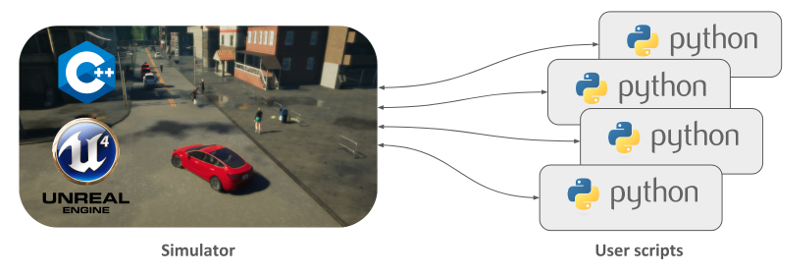
\includegraphics[width=1\linewidth]{Figures/Methods/carla_modules.png}
\caption{CARLA client-server architecture, where the Simulator is provided on the server side, and scripts can control the simulator on the client side}
\label{fig:carla_modules}
\end{figure}

The client-side of the architecture comprises numerous client modules, each controlling the logic of the actors in the scene and determining the world's conditions. The interaction between the server and client is facilitated by the CARLA API, available in Python or C++, which serves as an intermediary layer. This API is continually updated to offer new functionalities, enhancing the overall capabilities of the CARLA simulator.

The basic structure of CARLA can be summarised as:

\begin{itemize}
\item \textbf{Traffic Manager:} This is an integrated system in CARLA that manages the control of all vehicles excluding the one used for learning. It functions as a conductor to mimic realistic behaviours in urban-like environments.
\item \textbf{Sensors:} These are essential components for vehicles to gather information about their environment. In CARLA, sensors are a unique type of actor attached to the vehicle, and the data they collect can be accessed and stored for convenience. CARLA supports a range of sensors, including cameras, radars, lidars, and more.
\item \textbf{Recorder:} This tool allows for the step-by-step recreation of a simulation for every actor in the world. It provides access to any moment in the timeline at any location, making it a powerful tracing tool.
\item \textbf{ROS Bridge and Autoware Implementation:} In the pursuit of universal applicability, the CARLA project actively seeks to integrate the simulator within other learning environments.
\item \textbf{Open Assets:} CARLA provides various maps for urban settings, complete with control over weather conditions and a blueprint library containing a broad range of actors. These assets can be customized, and new ones can be created following simple guidelines.
\item \textbf{Scenario Runner:} To streamline the learning process for vehicles, CARLA provides a series of routes that describe different situations to iterate on. These routes also form the foundation for the CARLA challenge, an open competition for everyone to test their solutions and aim for a spot on the leaderboard.
\end{itemize}
%\%include{Chapters/04-Results}
%%%%%%%%%%%%%%%%%
%% DISCUSSION %%
%%%%%%%%%%%%%%%%

%This chapter examines your results in comparison with your objectives, and then in the wider perspective of other theoretical and applied work relevant to your project, as covered in your review in Chapter 2. For instance, for a software product you will discuss how well it satisfies the user needs that it addresses, its performance and dependability, aspects of design, implementation or assessment that have proved good choices or that instead you would change if you were to repeat the project knowing what you now know. For novel research results or any other knowledge obtained through the project, you will discuss your confidence in the results, their validity, scope and their generalisability. What are the implications of what you have found out? Do you have any recommendations as a result?

\chapter{Discussion}
\label{Discussion} 


%%%%%%%%%%%%%%%%%%%%%%%%%%%%%%%%%%%%%%%%%%%%%
% EVALUATION, REFLECTIONS AND CONCLUSIONS %%
%%%%%%%%%%%%%%%%%%%%%%%%%%%%%%%%%%%%%%%%%%%%

%This chapter should evaluate the project work as a whole. Here the original choice of objectives, the literature examined, the methods used, the planning, etc. are all reviewed to see what has been achieved by undertaking the project. There may be a summary of general conclusions drawn from the work done, highlighting the particular contribution of your project. You should also consider the implications of these conclusions. Discuss any proposals that you might make for further work, having discovered what you now know. It is also important to include a reflective section covering what you have learned from the project process. What would you do differently if you were to start again, knowing what you now know? Your report MUST include adequate Evaluation, Reflections and Conclusions to gain a passing grade. 

\chapter{Evaluation, Reflections and Conclusions}
\label{Eval}


%% Appendix A
% For referencing this appendix elsewhere, use \ref{AppendixA}
\chapter{Methods} % Main appendix title
\label{Appendix-methods} 

\section{AirSim}

This section describes installing AirSim on Ubuntu 20.04.


% \chapter{Results} % Main appendix title
\label{Appendix-results} % For referencing this appendix elsewhere, use 
In this chapter we document results, based on the methodology used.

\section{CARLA Simulator results}
In this section we document simulation results, describing the code repository commit hash, and any relevant commands and outputs.
%%%%%%%%%%%%%%%%%%%%%%%%%%%%%%%%%%%%%%%%%%%%%%%%%%%%%%%%%%%%%%%%%%%%%%%%%%%%%
% RUN XXX - TEMPLATE - experiment log template
%%%%%%%%%%%%%%%%%%%%%%%%%%%%%%%%%%%%%%%%%%%%%%%%%%%%%%%%%%%%%%%%%%%%%%%%%%%%%
%\subsection{Run XXX -  }
%\label{app_res:XXX}
%\begin{verbatim}
%Commit:
%Model: 
%Outputs: 
%Dataset: 
%Command:
%Environment: 
%Comment: 
%\end{verbatim}

%%%%%%%%%%%%%%%%%%%%%%%%%%%%%%%%%%%%%%%%%%%%%%%%%%%%%%%%%%%%%%%%%%%%%%%%%%%%%
% RUN 001 - Running CARLA
%%%%%%%%%%%%%%%%%%%%%%%%%%%%%%%%%%%%%%%%%%%%%%%%%%%%%%%%%%%%%%%%%%%%%%%%%%%%%
\subsection{Run 001 - Running Carla}
\label{app_res:001}
\begin{verbatim}
Commit: bb4b95e0
Environment: Local desktop
Command:
$ make launch-only

Comment:
Simulator loads ok.

\end{verbatim}

%%%%%%%%%%%%%%%%%%%%%%%%%%%%%%%%%%%%%%%%%%%%%%%%%%%%%%%%%%%%%%%%%%%%%%%%%%%%%
% RUN 002 - Adding actors
%%%%%%%%%%%%%%%%%%%%%%%%%%%%%%%%%%%%%%%%%%%%%%%%%%%%%%%%%%%%%%%%%%%%%%%%%%%%%
\subsection{Run 002 - Adding actors}
\label{app_res:002}
\begin{verbatim}
Commit: bb4b95e0
Environment: Local desktop
Command:
$ make launch-only
# In another terminal, change directory to PythonAPI/examples, and run
$ python generate_traffic.py 
spawned 30 vehicles and 10 walkers, press Ctrl+C to exit.

Comment:
Simulator loads ok. The  default number of spawned vehicles is 30 and pedestrians (walkers) is 10. To change and other options, see script for details. The defaults in this case can be changed by adding switches:
$ python generate_traffic.py -n 60 -w 100
\end{verbatim}

\begin{figure}[h!]
\centering
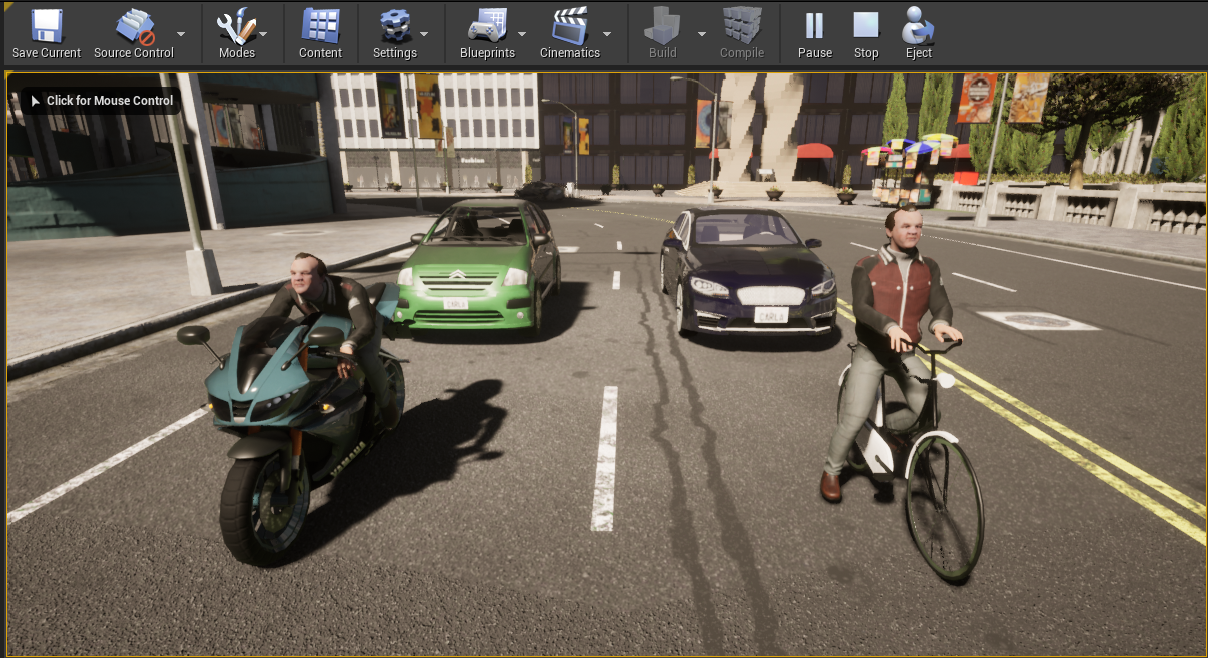
\includegraphics[width=\textwidth]{Figures/biker-cyclist.png}
\caption{CARLA simulator added actors}
\label{fig:biker-cyclist}
\end{figure}


%%%%%%%%%%%%%%%%%%%%%%%%%%%%%%%%%%%%%%%%%%%%%%%%%%%%%%%%%%%%%%%%%%%%%%%%%%%%%
% RUN 003 - Adding dynamic weather
%%%%%%%%%%%%%%%%%%%%%%%%%%%%%%%%%%%%%%%%%%%%%%%%%%%%%%%%%%%%%%%%%%%%%%%%%%%%%
\subsection{Run 003 - Adding dynamic weather}
\label{app_res:003}
\begin{verbatim}
Commit: bb4b95e0
Environment: Local desktop
Command:
$ make launch-only
# In another terminal, change directory to PythonAPI/examples, and run
$ python dynamic_weather.py -s 0.01
Sun(alt: -18.82, azm: 300.53) Storm(clouds=0%, rain=0%, wind=5%)            ^Z
[1]+  Stopped                 python3 dynamic_weather.py -s 0.01

Comment:
The parameter -s (speed) is a denominator in code, see
update_freq = 0.1 / speed_factor
The smaller the number, the less frequent (slower) are the weather updates, the greater the number, the more frequent (faster) are the weather updates.
\end{verbatim}

%%%%%%%%%%%%%%%%%%%%%%%%%%%%%%%%%%%%%%%%%%%%%%%%%%%%%%%%%%%%%%%%%%%%%%%%%%%%%
% RUN 004 - Automatic control
%%%%%%%%%%%%%%%%%%%%%%%%%%%%%%%%%%%%%%%%%%%%%%%%%%%%%%%%%%%%%%%%%%%%%%%%%%%%%
\subsection{Run 004 - Automatic control}
\label{app_res:004}
\begin{verbatim}
Commit: bb4b95e0
Environment: Local desktop
Date: 2021.11.21
Command:
$ make launch-only
# Once loaded, press play
# In another terminal, change directory to PythonAPI/examples, and run
$ python automatic_control.py

Comment:
This launches a pygame terminal, with a random vehicle set to ran
\end{verbatim}

%%%%%%%%%%%%%%%%%%%%%%%%%%%%%%%%%%%%%%%%%%%%%%%%%%%%%%%%%%%%%%%%%%%%%%%%%%%%%
% RUN 005 - Automatic control with traffic
%%%%%%%%%%%%%%%%%%%%%%%%%%%%%%%%%%%%%%%%%%%%%%%%%%%%%%%%%%%%%%%%%%%%%%%%%%%%%
\subsection{Run 005 - Automatic control with traffic}
\label{app_res:005}
\begin{verbatim}
Commit: bb4b95e0
Environment: Local desktop
Date: 2021.11.21
Command:
$ make launch-only
# Once loaded, press play
# In another terminal, change directory to PythonAPI/examples, and run
$ python generate_traffic.py 
spawned 30 vehicles and 10 walkers, press Ctrl+C to exit.

# In another terminal, change directory to PythonAPI/examples, and run
$ python automatic_control.py

Comment:
Traffic and automatic control vehicle are visible both in the pygame and unreal 
engine screens.
\end{verbatim}

%%%%%%%%%%%%%%%%%%%%%%%%%%%%%%%%%%%%%%%%%%%%%%%%%%%%%%%%%%%%%%%%%%%%%%%%%%%%%
% RUN 006 - Automatic control with traffic and dynamic weather
%%%%%%%%%%%%%%%%%%%%%%%%%%%%%%%%%%%%%%%%%%%%%%%%%%%%%%%%%%%%%%%%%%%%%%%%%%%%%
\subsection{Run 006- Automatic control with traffic and dynamic weather}
\label{app_res:006}
\begin{verbatim}
Commit: bb4b95e0
Environment: Local desktop
Date: 2021.11.21
Command:
$ make launch-only
# Once loaded, press play
# In another terminal, change directory to PythonAPI/examples, and run
$ python generate_traffic.py 
spawned 30 vehicles and 10 walkers, press Ctrl+C to exit.

# In another terminal, change directory to PythonAPI/examples, and run
$ python dynamic_weather.py -s 0.05
Sun(alt: -19.78, azm: 300.10) Storm(clouds=0%, rain=0%, wind=5%)  

# In another terminal, change directory to PythonAPI/examples, and run
$ python automatic_control.py

Comment:
The sun position changes every two seconds when parameter -s 0.05 is 
passed (0.1 / 0.05 = 2)

To exit the simulation:
1. Ensure dynamic_weather.py is not running or stop with CONTROL + C
2. Stop generate_traffic.py with CONTROL + C
3. Stop dynamic_weather.py with CONTROL + C
4. Stop Unreal Engine

If script generate_traffic.py is not stopped with CONTROL + C, and say CONTROL + Z, may still be running in the background. This will keep a lock on the port.

To list processes (open files) that have port 2000 open:
$ sudo lsof -t -i:2000
3281
3416

To check which process the process ID listed refers to:
$ ps aux | grep 3281
daniel    3281  0.9  0.2 1860476 90348 pts/1   Tl   17:25   0:29 python3 generate_traffic.py
daniel    7455  0.0  0.0  14432  1040 pts/1    S+   18:18   0:00 grep --color=auto 3281

To kill the process:
$ sudo kill -9 3281
[1]+  Killed                  python3 generate_traffic.py

\end{verbatim}

\begin{figure}[h!]
\centering
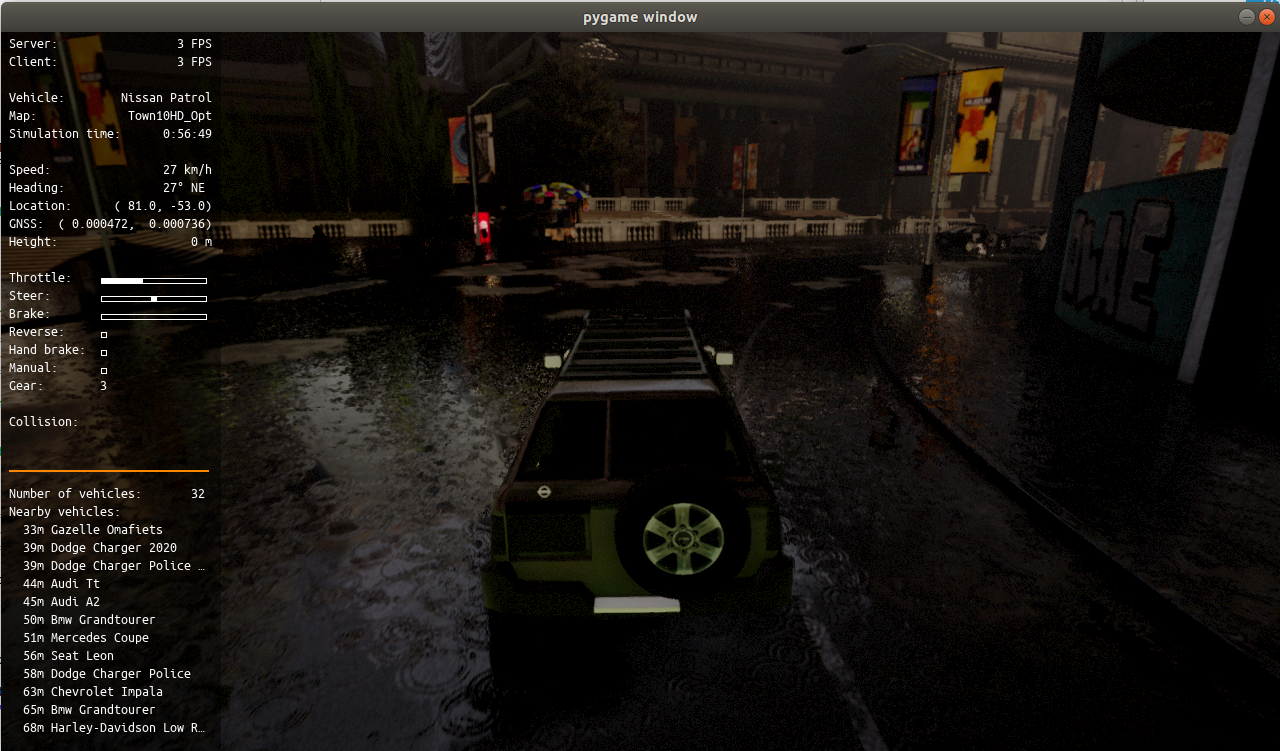
\includegraphics[width=\textwidth]{Figures/carla-rain.png}
\caption{CARLA simulator with dynamic weather}
\label{fig:carla-rain}
\end{figure}

\begin{figure}[h!]
\centering
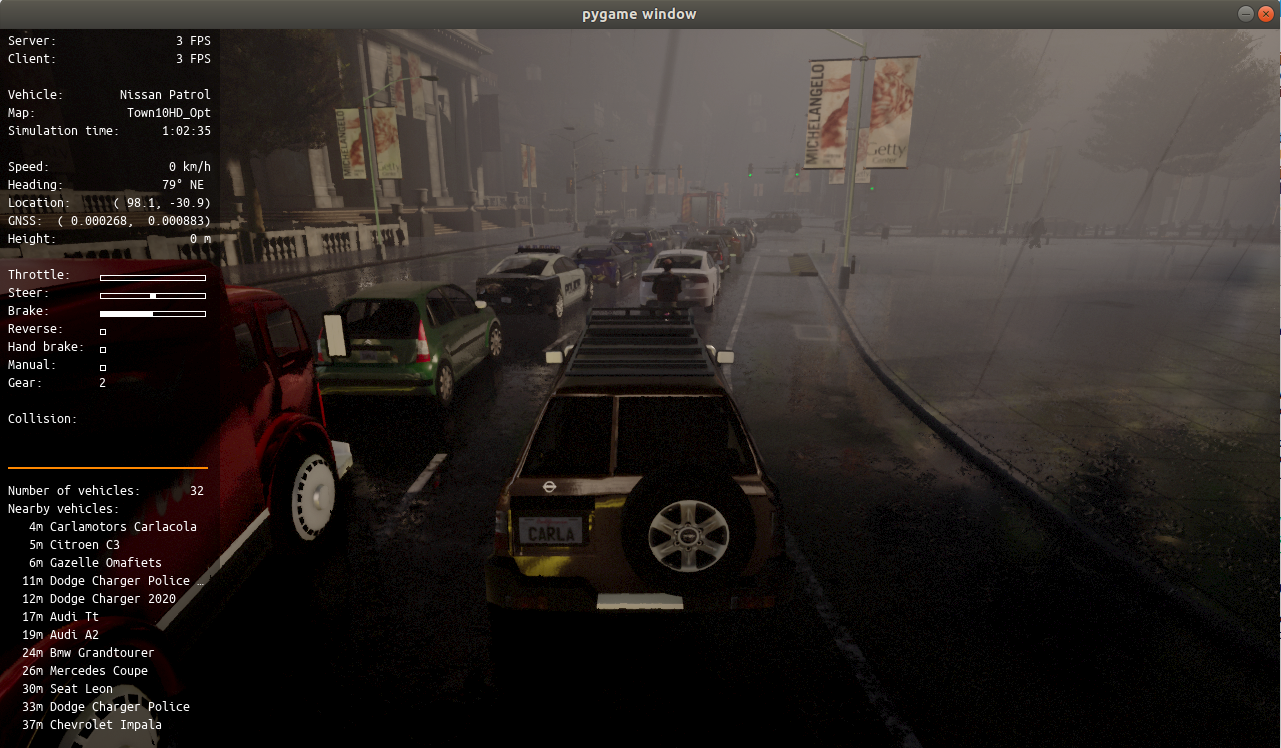
\includegraphics[width=\textwidth]{Figures/carla-traffic-jam.png}
\caption{CARLA simulator traffic jam}
\label{fig:carla-traffic-jam}
\end{figure}

Figures \ref{fig:carla-rain} and \ref{fig:carla-traffic-jam} are taken from the pygame screen.

\begin{figure}[h!]
\centering
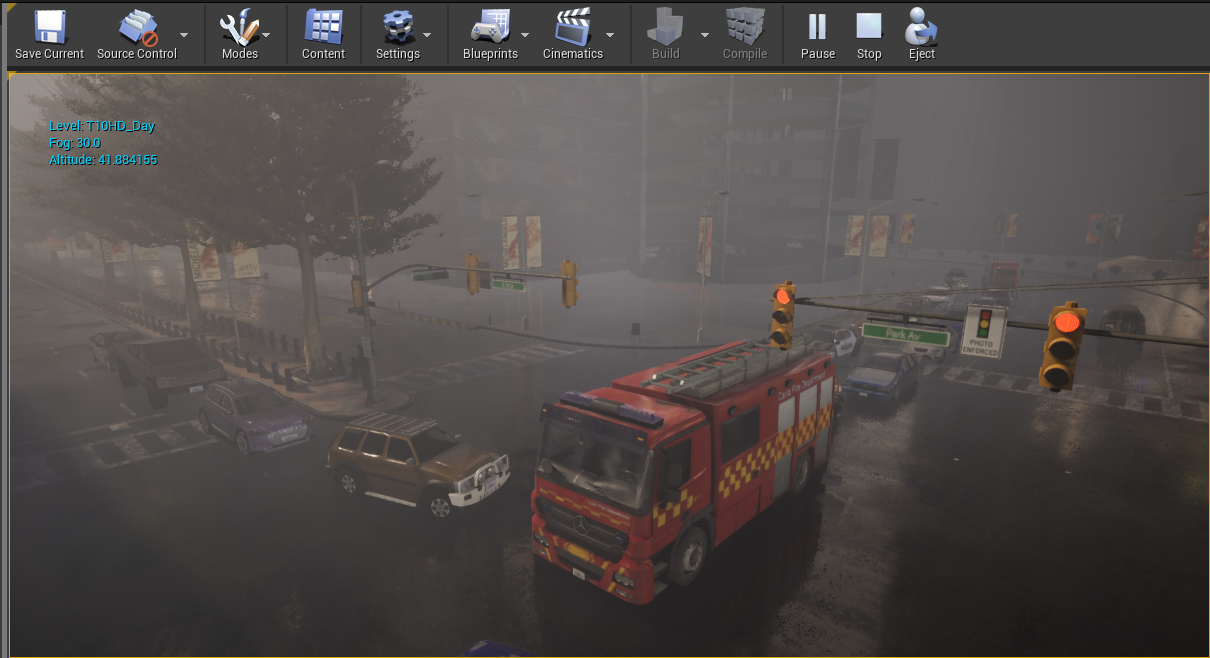
\includegraphics[width=\textwidth]{Figures/carla-traffic-jam-2.png}
\caption{CARLA simulator traffic jam reverse angle}
\label{fig:carla-traffic-jam-2}
\end{figure}

Figure \ref{fig:carla-traffic-jam-2}, taken from Unreal Engine, showing the stopped vehicles at the T-junction and is the reverse angle of Figure \ref{fig:carla-traffic-jam}. note there has not been a collision. The algorithm driving each vehicle seems to be stuck by a proximity assessment that is unlikely to change given all vehicles are stopped.

%%%%%%%%%%%%%%%%%%%%%%%%%%%%%%%%%%%%%%%%%%%%%%%%%%%%%%%%%%%%%%%%%%%%%%%%%%%%%
% RUN 007 - Automatic control with traffic
%%%%%%%%%%%%%%%%%%%%%%%%%%%%%%%%%%%%%%%%%%%%%%%%%%%%%%%%%%%%%%%%%%%%%%%%%%%%%
\subsection{Run 007- Automatic control with traffic}
\label{app_res:007}
\begin{verbatim}
Commit: bb4b95e0
Environment: Local desktop
Date: 2021.11.22
Commands:
$ make launch-only
# Loaded Town04_Opt
$ python generate_traffic.py -n 60 -w 600
spawned 60 vehicles and 328 walkers, press Ctrl+C to exit.
# NB some walkers not created due to collisions
# In another terminal, change directory to PythonAPI/examples, and run
$ python automatic_control.py

Comment:
Various successive runs, number of vehicles decreasing over time due to collisions. One simulated self-drving vehicle got stuck in the simulation (tipycally it would be destroyed at the end of self-driving simulation) after crashing against a traffic-light post.
\end{verbatim}

%%%%%%%%%%%%%%%%%%%%%%%%%%%%%%%%%%%%%%%%%%%%%%%%%%%%%%%%%%%%%%%%%%%%%%%%%%%%%
% RUN 008 - Using the same vehicle
%%%%%%%%%%%%%%%%%%%%%%%%%%%%%%%%%%%%%%%%%%%%%%%%%%%%%%%%%%%%%%%%%%%%%%%%%%%%%
\subsection{Run 008 - Using the same vehicle}
\label{app_res:008}
\begin{verbatim}
Commit: bb4b95e0
Environment: Local desktop
Date: 2021.12.05
Commands:
$ make launch-only
# Loaded Town10HD_Opt (current default)
# pressed "Play"
# generated dynamic weather
$ python dynamic_weather.py --speed 0.1
# generate traffic
$ python generate_traffic.py -n 60 -w 600
(...)
Vehicle agent not added to the crowd by some problem!
(...)
# error message assumed to caused by starting sequence i.e. dynamic weather before dynamic traffic.
$ python generate_traffic.py -n 60 -w 600

Comment:
Currently code uses a random vehicle chosen in automatic_control.py. All cars vanished from simulation two hours in. Pedestrians still present.
\end{verbatim}


%%%%%%%%%%%%%%%%%%%%%%%%%%%%%%%%%%%%%%%%%%%%%%%%%%%%%%%%%%%%%%%%%%%%%%%%%%%%%
% RUN 009 - Hyperion test
%%%%%%%%%%%%%%%%%%%%%%%%%%%%%%%%%%%%%%%%%%%%%%%%%%%%%%%%%%%%%%%%%%%%%%%%%%%%%
\subsection{Run 009 - Hyperion High Computing Cluster Test}
\label{app_res:009}
\begin{verbatim}
Repository: https://github.com/dsikar/mscai
Branch: master
Commit: d4409a20
Environment: Hyperion
Date: 2022.03.20
Connection details:
As per "HPC - How to connect using windows"
Commands:
$ cd ~/localscratch 
$ git clone https://github.com/dsikar/mscai
$ cd Lab1
# deactivate environment - activated by default in ~/.bashrc
$ flight env deactivate
# run
$ source /opt/flight/etc/setup.sh
$ flight env activate singularity
$ singularity exec --nv /mnt/scratch/singularity/psarin/ubuntu20_04cuda11.sif \  /usr/bin/python3 /users/aczd097/localscratch/mscai/Lab1/DLIALab1.py

Comment:
This script is supposed to run with 
aczd097@login1 ~/localscratch/mscai/Lab1 (master)$ sbatch runModel.sh
Submitted batch job 173522

The JOBID does not appear in the queue. Assumption is job fails to start.

from: https://sylabs.io/guides/3.7/user-guide/definition_files.html
The process of creating the singularity container (.sif file) is:

1. A script is created:
/mnt/scratch/singularity/psarin/ubuntu20_04cuda11.def
2. And built:
$ sudo singularity build --notest my_container.sif my_container.def

\end{verbatim}


%%%%%%%%%%%%%%%%%%%%%%%%%%%%%%%%%%%%%%%%%%%%%%%%%%%%%%%%%%%%%%%%%%%%%%%%%%%%%
% RUN XXX - Template
%%%%%%%%%%%%%%%%%%%%%%%%%%%%%%%%%%%%%%%%%%%%%%%%%%%%%%%%%%%%%%%%%%%%%%%%%%%%%
\subsection{Run XXX - Template}
\label{app_res:XXX}
\begin{verbatim}
Commit: bb4b95e0
Environment: Local desktop
Date: 2021.12.05
Commands:
$ make launch-only
# Loaded Town10HD_Opt (current default)
# pressed "Play"
# generated dynamic weather
$ python dynamic_weather.py --speed 0.1
# generate traffic
$ python generate_traffic.py -n 60 -w 600
(...)
Vehicle agent not added to the crowd by some problem!
(...)
# error message assumed to caused by starting sequence i.e. dynamic weather before dynamic traffic.
$ python generate_traffic.py -n 60 -w 600

Comment:
Currently code uses a random vehicle chosen in automatic_control.py. All cars vanished from simulation two hours in. Pedestrians still present.
\end{verbatim}

%% Appendix Template
\chapter{Meeting minutes}

\label{Appendix-meeting-minutes} % label e.g. Appendix-results 

%%%%%%%%%%%%%%%%%%%%%%%%%%%%%%%%%%%%%%%%%%%%%%%%%%%%%%%%%%%%%%%%%%%%%%%%%%%%%
% Meeting Minutes XXX - TEMPLATE
%%%%%%%%%%%%%%%%%%%%%%%%%%%%%%%%%%%%%%%%%%%%%%%%%%%%%%%%%%%%%%%%%%%%%%%%%%%%%
%\subsection{Meeting Minutes XXX}
%\label{meeting_minutes:XXX}

\large
\textbf{Intel ICSR Sync Meeting Minutes 2021.07.10}
\vspace{0.23cm}

\begin{tabular}{ll}
Location:  & Google Meet \\
Date: &  2021.07.10 \\ 
Time: & 1600h UTC+1 \\ 
Attendees: & R. Bloomfield \\
 & R. Aghadezadeh Chakherlou, \\
 & P. Popov, \\
 & D. Sikar, \\
 & M. Stewart,  \\
 & L. Stringini \\ 
\end{tabular}
\vspace{0.23cm}

\textbf{Agenda items}
\vspace{0.23cm}

\begin{itemize}
    \item 1. RB briefly described the trade-off between reasoning (depth of detail) and communication (breadth of reach) which assurance cases. Using AI to explain assurance and vice-versa. Differences in assurance cases used in Europe vs US, outcome based, where the goals that have to be met are given (problem is it can be too vague). Prescriptive - "this is what the system needs to do", respectively.
    \item 2. PP briefly described the concept of fragments and substitution, claims about real world, is car safe (define what safe is) substitute with related claim, obligations, defeaters. Suggested I look through SAFECOMP papers e.g. "Computer Safety, Reliability, and Security: SAFECOMP 2014 Workshops: ASCoMS, DECSoS, DEVVARTS, ISSE, ReSA4CI, SASSUR. Florence, Italy, September 8-9, 2014. Proceedings", , Other concept to look into: "digital twins".
    \item 3. RB suggests we (RAC, DS, MS) prepare a couple of "progress" slides for the next ICSR Sync Meeting (2020.08.05).
    \item 4. LS defined the the scope of RAC's current research: to "organise evidence of the arguments"
    \item 5. RAC posted in the chat a link to "Safety Case Templates for Autonomous Systems" 
\end{itemize}

\textbf{Follow-up links}
\vspace{0.23cm}
   %\Url{https://bit.ly/3AOiM43}
% [2] "Safety Case Templates for Autonomous Systems" \Url{https://arxiv.org/abs/2102.02625}.

\begin{tabular}{ll}
1 & \href{https://bit.ly/3AOiM43}{SAFECOMP 2014} \\
2 & \href{https://arxiv.org/abs/2102.02625}{Safety Case Templates for Autonomous Systems} \\
3 & \href{Assurance 2.0: A Manifesto}{https://arxiv.org/pdf/2004.10474.pdf} \\
4 & \href{https://ico.org.uk/for-organisations/guide-to-data-protection/key-data-protection-themes/explaining-decisions-made-with-artificial-intelligence/}{Explaining decisions made with AI} \\
5 & 

% ICO 
% The UK’s independent authority set up to uphold information rights in the public interest, promoting openness by public bodies and data privacy for individuals.

% ICO 3 key dev areas:
% Information Commissioner’s Office
% Technology Strategy2018-2021
% https://ico.org.uk/media/about-the-ico/documents/2258299/ico-technology-strategy-2018-2021.pdf
% We will establish Technology Fellowships for post-doctoral experts to enable us to increase our in-house advice and expertise on technology priority areas. Our first appointment will bea two-year post-doctoral role toinvestigate and research the impact of artificial intelligence on data privacy, encompassing big data and machine learning.

% Following on from our successful report on the data protection implications of Artificial Intelligence (AI) and machine learning will produce further reportson emerging technology issues.

% Commissioner’s message - Technology is driving changes to the societal, political, legal and business environment that the Information Commissioner’s Office (ICO)needs to regulate. The most significant data protection risks to individuals are now driven by the use of new technologies.The risks are broad –from cyber-attacksto the growth of artificial intelligence and machine learning

\end{tabular}

TODO Action points
% Action items  % Owner(s) % Deadline % Status 
%Further todos
% 1. meeting minutes - In progress
% 2. article (MSc results)
% 4. Carla Autoware setup

%----------------------------------------------------------------------------------------
%	BIBLIOGRAPHY
%----------------------------------------------------------------------------------------

\printbibliography[heading=bibintoc]

%----------------------------------------------------------------------------------------

%----------------------------------------------------------------------------------------
%	THESIS CONTENT - APPENDICES
%----------------------------------------------------------------------------------------


\appendix % Cue to tell LaTeX that the following "chapters" are Appendices

% Appendix page numbering
\pretocmd{\chapter}{%
  \clearpage
  \pagenumbering{arabic}%
  \renewcommand*{\thepage}{\thechapter\arabic{page}}%
}{}{}

% Include the appendices of the thesis as separate files from the Appendices folder
% Uncomment the lines as you write the Appendices

\begin{appendices}

%% Appendix 0 - RPMI Project

% Note: this appendix is a .pdf document, placed
% in the top level of project directory
%\chapter{RPMI Project Proposal Proposal} % Main appendix title
\label{app:rpmi}
% RPMI Project Proposal to be included. 
%\includepdf[page={1-9}]{Sikar_D_RPMI_Task2_v7}


%% Appendix A
% For referencing this appendix elsewhere, use \ref{AppendixA}
\chapter{Methods} % Main appendix title
\label{Appendix-methods} 


%\chapter{Results} % Main appendix title
\label{Appendix-results} % For referencing this appendix elsewhere, use 
In this chapter we document results, based on the methodology used.

\section{CARLA Simulator results}
In this section we document simulation results, describing the code repository commit hash, and any relevant commands and outputs.
%%%%%%%%%%%%%%%%%%%%%%%%%%%%%%%%%%%%%%%%%%%%%%%%%%%%%%%%%%%%%%%%%%%%%%%%%%%%%
% RUN XXX - TEMPLATE - experiment log template
%%%%%%%%%%%%%%%%%%%%%%%%%%%%%%%%%%%%%%%%%%%%%%%%%%%%%%%%%%%%%%%%%%%%%%%%%%%%%
%\subsection{Run XXX -  }
%\label{app_res:XXX}
%\begin{verbatim}
%Commit:
%Model: 
%Outputs: 
%Dataset: 
%Command:
%Environment: 
%Comment: 
%\end{verbatim}

%%%%%%%%%%%%%%%%%%%%%%%%%%%%%%%%%%%%%%%%%%%%%%%%%%%%%%%%%%%%%%%%%%%%%%%%%%%%%
% RUN 001 - Running CARLA
%%%%%%%%%%%%%%%%%%%%%%%%%%%%%%%%%%%%%%%%%%%%%%%%%%%%%%%%%%%%%%%%%%%%%%%%%%%%%
\subsection{Run 001 - Running Carla}
\label{app_res:001}
\begin{verbatim}
Commit: bb4b95e0
Environment: Local desktop
Command:
$ make launch-only

Comment:
Simulator loads ok.

\end{verbatim}

%%%%%%%%%%%%%%%%%%%%%%%%%%%%%%%%%%%%%%%%%%%%%%%%%%%%%%%%%%%%%%%%%%%%%%%%%%%%%
% RUN 002 - Adding actors
%%%%%%%%%%%%%%%%%%%%%%%%%%%%%%%%%%%%%%%%%%%%%%%%%%%%%%%%%%%%%%%%%%%%%%%%%%%%%
\subsection{Run 002 - Adding actors}
\label{app_res:002}
\begin{verbatim}
Commit: bb4b95e0
Environment: Local desktop
Command:
$ make launch-only
# In another terminal, change directory to PythonAPI/examples, and run
$ python generate_traffic.py 
spawned 30 vehicles and 10 walkers, press Ctrl+C to exit.

Comment:
Simulator loads ok. The  default number of spawned vehicles is 30 and pedestrians (walkers) is 10. To change and other options, see script for details. The defaults in this case can be changed by adding switches:
$ python generate_traffic.py -n 60 -w 100
\end{verbatim}

\begin{figure}[h!]
\centering
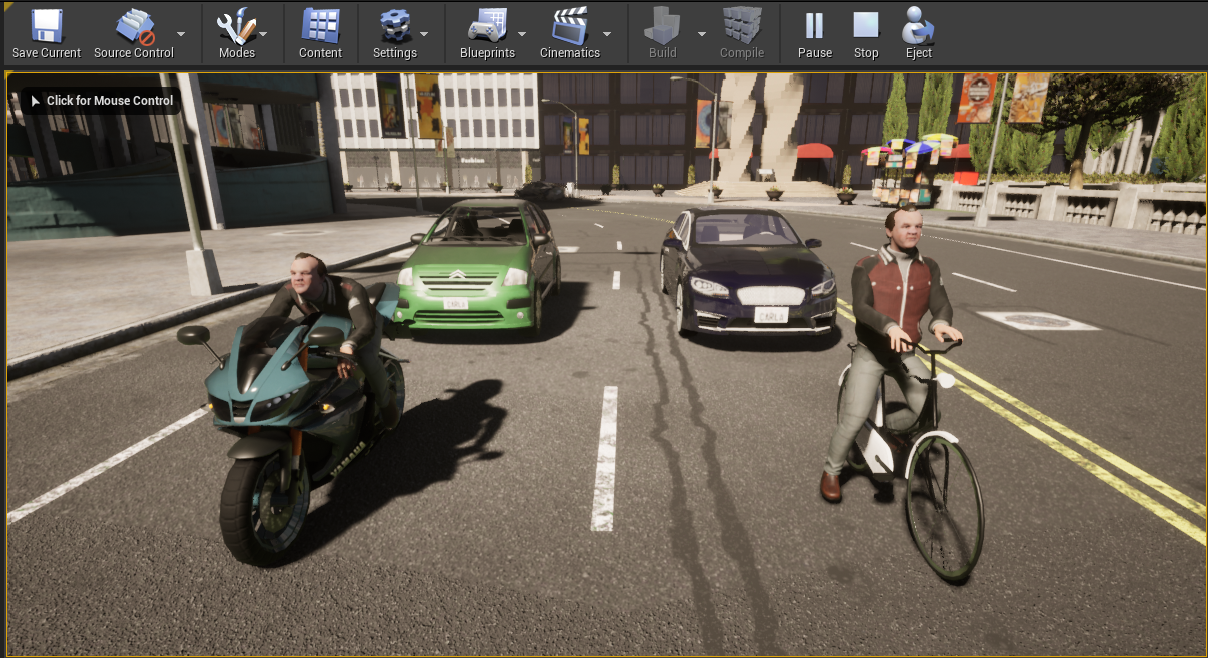
\includegraphics[width=\textwidth]{Figures/biker-cyclist.png}
\caption{CARLA simulator added actors}
\label{fig:biker-cyclist}
\end{figure}


%%%%%%%%%%%%%%%%%%%%%%%%%%%%%%%%%%%%%%%%%%%%%%%%%%%%%%%%%%%%%%%%%%%%%%%%%%%%%
% RUN 003 - Adding dynamic weather
%%%%%%%%%%%%%%%%%%%%%%%%%%%%%%%%%%%%%%%%%%%%%%%%%%%%%%%%%%%%%%%%%%%%%%%%%%%%%
\subsection{Run 003 - Adding dynamic weather}
\label{app_res:003}
\begin{verbatim}
Commit: bb4b95e0
Environment: Local desktop
Command:
$ make launch-only
# In another terminal, change directory to PythonAPI/examples, and run
$ python dynamic_weather.py -s 0.01
Sun(alt: -18.82, azm: 300.53) Storm(clouds=0%, rain=0%, wind=5%)            ^Z
[1]+  Stopped                 python3 dynamic_weather.py -s 0.01

Comment:
The parameter -s (speed) is a denominator in code, see
update_freq = 0.1 / speed_factor
The smaller the number, the less frequent (slower) are the weather updates, the greater the number, the more frequent (faster) are the weather updates.
\end{verbatim}

%%%%%%%%%%%%%%%%%%%%%%%%%%%%%%%%%%%%%%%%%%%%%%%%%%%%%%%%%%%%%%%%%%%%%%%%%%%%%
% RUN 004 - Automatic control
%%%%%%%%%%%%%%%%%%%%%%%%%%%%%%%%%%%%%%%%%%%%%%%%%%%%%%%%%%%%%%%%%%%%%%%%%%%%%
\subsection{Run 004 - Automatic control}
\label{app_res:004}
\begin{verbatim}
Commit: bb4b95e0
Environment: Local desktop
Date: 2021.11.21
Command:
$ make launch-only
# Once loaded, press play
# In another terminal, change directory to PythonAPI/examples, and run
$ python automatic_control.py

Comment:
This launches a pygame terminal, with a random vehicle set to ran
\end{verbatim}

%%%%%%%%%%%%%%%%%%%%%%%%%%%%%%%%%%%%%%%%%%%%%%%%%%%%%%%%%%%%%%%%%%%%%%%%%%%%%
% RUN 005 - Automatic control with traffic
%%%%%%%%%%%%%%%%%%%%%%%%%%%%%%%%%%%%%%%%%%%%%%%%%%%%%%%%%%%%%%%%%%%%%%%%%%%%%
\subsection{Run 005 - Automatic control with traffic}
\label{app_res:005}
\begin{verbatim}
Commit: bb4b95e0
Environment: Local desktop
Date: 2021.11.21
Command:
$ make launch-only
# Once loaded, press play
# In another terminal, change directory to PythonAPI/examples, and run
$ python generate_traffic.py 
spawned 30 vehicles and 10 walkers, press Ctrl+C to exit.

# In another terminal, change directory to PythonAPI/examples, and run
$ python automatic_control.py

Comment:
Traffic and automatic control vehicle are visible both in the pygame and unreal 
engine screens.
\end{verbatim}

%%%%%%%%%%%%%%%%%%%%%%%%%%%%%%%%%%%%%%%%%%%%%%%%%%%%%%%%%%%%%%%%%%%%%%%%%%%%%
% RUN 006 - Automatic control with traffic and dynamic weather
%%%%%%%%%%%%%%%%%%%%%%%%%%%%%%%%%%%%%%%%%%%%%%%%%%%%%%%%%%%%%%%%%%%%%%%%%%%%%
\subsection{Run 006- Automatic control with traffic and dynamic weather}
\label{app_res:006}
\begin{verbatim}
Commit: bb4b95e0
Environment: Local desktop
Date: 2021.11.21
Command:
$ make launch-only
# Once loaded, press play
# In another terminal, change directory to PythonAPI/examples, and run
$ python generate_traffic.py 
spawned 30 vehicles and 10 walkers, press Ctrl+C to exit.

# In another terminal, change directory to PythonAPI/examples, and run
$ python dynamic_weather.py -s 0.05
Sun(alt: -19.78, azm: 300.10) Storm(clouds=0%, rain=0%, wind=5%)  

# In another terminal, change directory to PythonAPI/examples, and run
$ python automatic_control.py

Comment:
The sun position changes every two seconds when parameter -s 0.05 is 
passed (0.1 / 0.05 = 2)

To exit the simulation:
1. Ensure dynamic_weather.py is not running or stop with CONTROL + C
2. Stop generate_traffic.py with CONTROL + C
3. Stop dynamic_weather.py with CONTROL + C
4. Stop Unreal Engine

If script generate_traffic.py is not stopped with CONTROL + C, and say CONTROL + Z, may still be running in the background. This will keep a lock on the port.

To list processes (open files) that have port 2000 open:
$ sudo lsof -t -i:2000
3281
3416

To check which process the process ID listed refers to:
$ ps aux | grep 3281
daniel    3281  0.9  0.2 1860476 90348 pts/1   Tl   17:25   0:29 python3 generate_traffic.py
daniel    7455  0.0  0.0  14432  1040 pts/1    S+   18:18   0:00 grep --color=auto 3281

To kill the process:
$ sudo kill -9 3281
[1]+  Killed                  python3 generate_traffic.py

\end{verbatim}

\begin{figure}[h!]
\centering
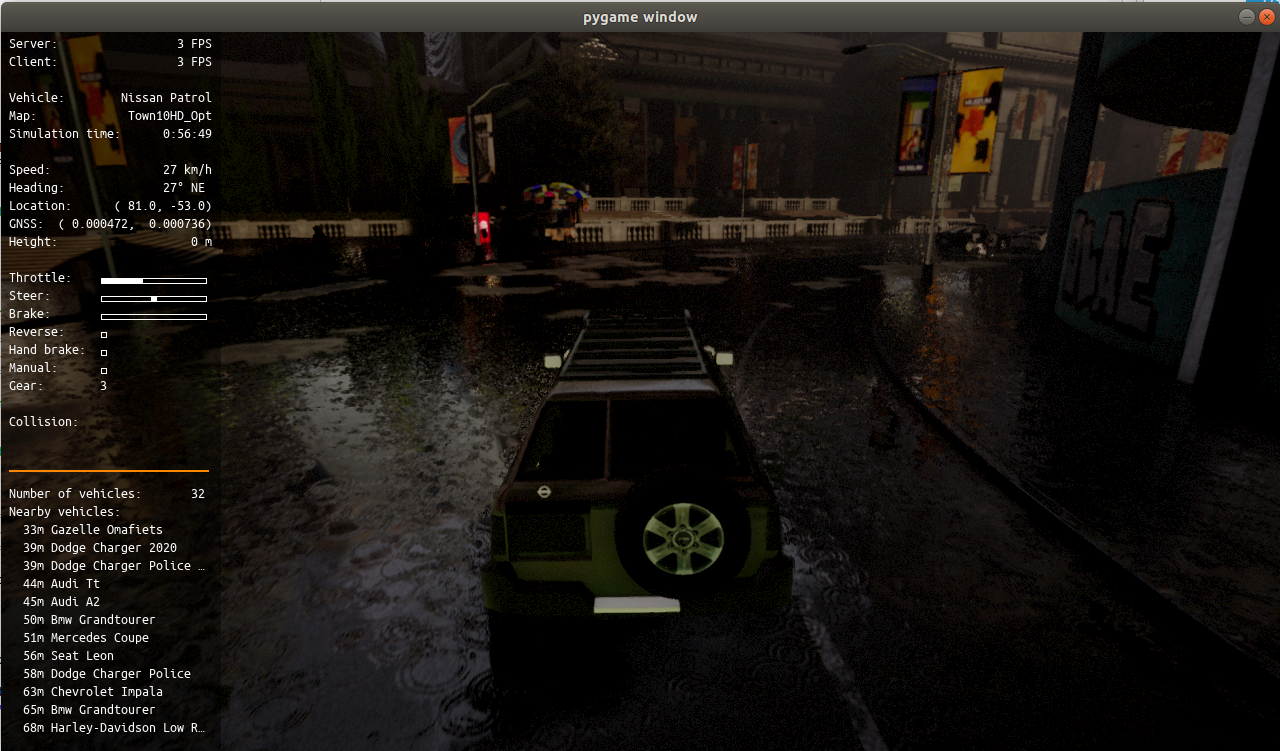
\includegraphics[width=\textwidth]{Figures/carla-rain.png}
\caption{CARLA simulator with dynamic weather}
\label{fig:carla-rain}
\end{figure}

\begin{figure}[h!]
\centering
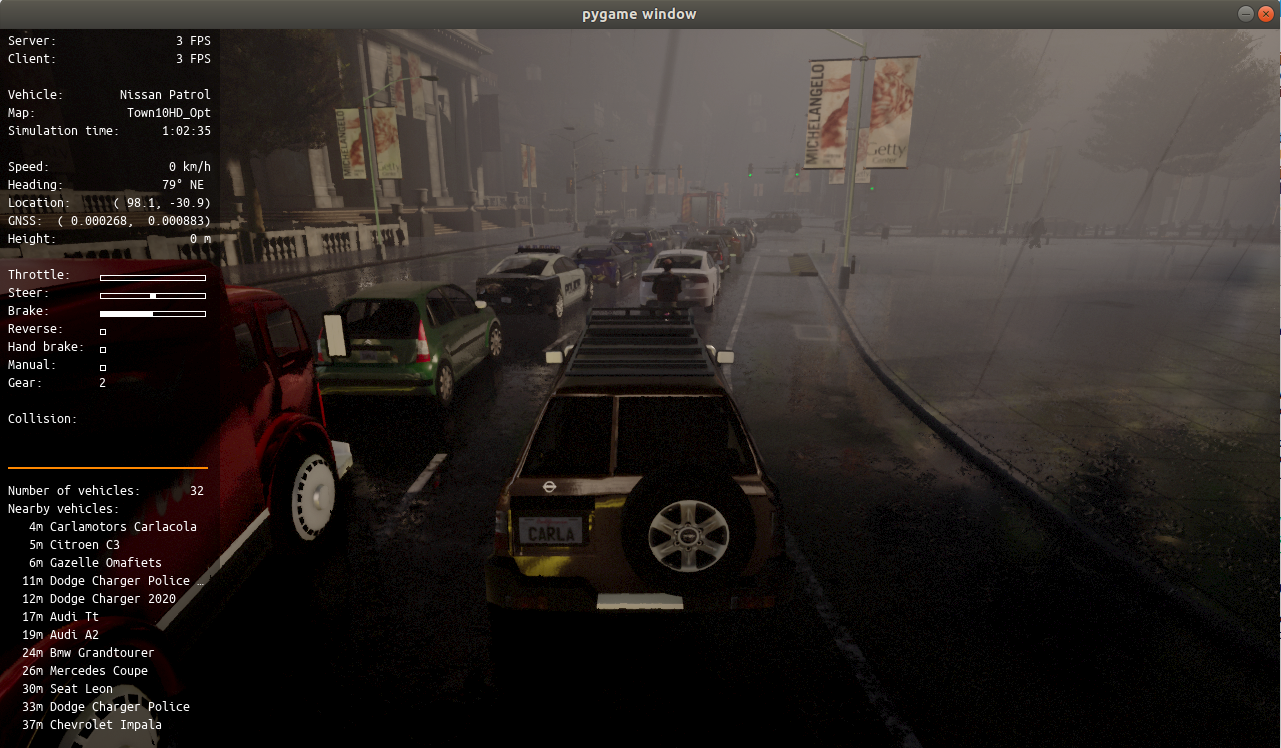
\includegraphics[width=\textwidth]{Figures/carla-traffic-jam.png}
\caption{CARLA simulator traffic jam}
\label{fig:carla-traffic-jam}
\end{figure}

Figures \ref{fig:carla-rain} and \ref{fig:carla-traffic-jam} are taken from the pygame screen.

\begin{figure}[h!]
\centering
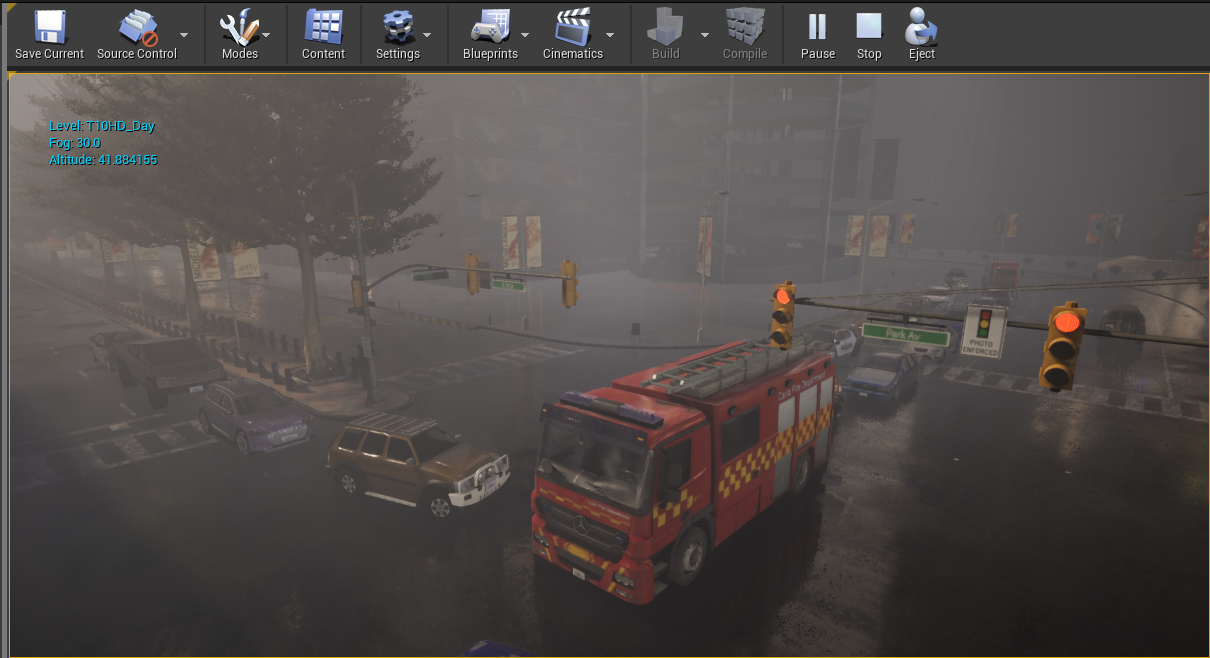
\includegraphics[width=\textwidth]{Figures/carla-traffic-jam-2.png}
\caption{CARLA simulator traffic jam reverse angle}
\label{fig:carla-traffic-jam-2}
\end{figure}

Figure \ref{fig:carla-traffic-jam-2}, taken from Unreal Engine, showing the stopped vehicles at the T-junction and is the reverse angle of Figure \ref{fig:carla-traffic-jam}. note there has not been a collision. The algorithm driving each vehicle seems to be stuck by a proximity assessment that is unlikely to change given all vehicles are stopped.

%%%%%%%%%%%%%%%%%%%%%%%%%%%%%%%%%%%%%%%%%%%%%%%%%%%%%%%%%%%%%%%%%%%%%%%%%%%%%
% RUN 007 - Automatic control with traffic
%%%%%%%%%%%%%%%%%%%%%%%%%%%%%%%%%%%%%%%%%%%%%%%%%%%%%%%%%%%%%%%%%%%%%%%%%%%%%
\subsection{Run 007- Automatic control with traffic}
\label{app_res:007}
\begin{verbatim}
Commit: bb4b95e0
Environment: Local desktop
Date: 2021.11.22
Commands:
$ make launch-only
# Loaded Town04_Opt
$ python generate_traffic.py -n 60 -w 600
spawned 60 vehicles and 328 walkers, press Ctrl+C to exit.
# NB some walkers not created due to collisions
# In another terminal, change directory to PythonAPI/examples, and run
$ python automatic_control.py

Comment:
Various successive runs, number of vehicles decreasing over time due to collisions. One simulated self-drving vehicle got stuck in the simulation (tipycally it would be destroyed at the end of self-driving simulation) after crashing against a traffic-light post.
\end{verbatim}

%%%%%%%%%%%%%%%%%%%%%%%%%%%%%%%%%%%%%%%%%%%%%%%%%%%%%%%%%%%%%%%%%%%%%%%%%%%%%
% RUN 008 - Using the same vehicle
%%%%%%%%%%%%%%%%%%%%%%%%%%%%%%%%%%%%%%%%%%%%%%%%%%%%%%%%%%%%%%%%%%%%%%%%%%%%%
\subsection{Run 008 - Using the same vehicle}
\label{app_res:008}
\begin{verbatim}
Commit: bb4b95e0
Environment: Local desktop
Date: 2021.12.05
Commands:
$ make launch-only
# Loaded Town10HD_Opt (current default)
# pressed "Play"
# generated dynamic weather
$ python dynamic_weather.py --speed 0.1
# generate traffic
$ python generate_traffic.py -n 60 -w 600
(...)
Vehicle agent not added to the crowd by some problem!
(...)
# error message assumed to caused by starting sequence i.e. dynamic weather before dynamic traffic.
$ python generate_traffic.py -n 60 -w 600

Comment:
Currently code uses a random vehicle chosen in automatic_control.py. All cars vanished from simulation two hours in. Pedestrians still present.
\end{verbatim}


%%%%%%%%%%%%%%%%%%%%%%%%%%%%%%%%%%%%%%%%%%%%%%%%%%%%%%%%%%%%%%%%%%%%%%%%%%%%%
% RUN 009 - Hyperion test
%%%%%%%%%%%%%%%%%%%%%%%%%%%%%%%%%%%%%%%%%%%%%%%%%%%%%%%%%%%%%%%%%%%%%%%%%%%%%
\subsection{Run 009 - Hyperion High Computing Cluster Test}
\label{app_res:009}
\begin{verbatim}
Repository: https://github.com/dsikar/mscai
Branch: master
Commit: d4409a20
Environment: Hyperion
Date: 2022.03.20
Connection details:
As per "HPC - How to connect using windows"
Commands:
$ cd ~/localscratch 
$ git clone https://github.com/dsikar/mscai
$ cd Lab1
# deactivate environment - activated by default in ~/.bashrc
$ flight env deactivate
# run
$ source /opt/flight/etc/setup.sh
$ flight env activate singularity
$ singularity exec --nv /mnt/scratch/singularity/psarin/ubuntu20_04cuda11.sif \  /usr/bin/python3 /users/aczd097/localscratch/mscai/Lab1/DLIALab1.py

Comment:
This script is supposed to run with 
aczd097@login1 ~/localscratch/mscai/Lab1 (master)$ sbatch runModel.sh
Submitted batch job 173522

The JOBID does not appear in the queue. Assumption is job fails to start.

from: https://sylabs.io/guides/3.7/user-guide/definition_files.html
The process of creating the singularity container (.sif file) is:

1. A script is created:
/mnt/scratch/singularity/psarin/ubuntu20_04cuda11.def
2. And built:
$ sudo singularity build --notest my_container.sif my_container.def

\end{verbatim}


%%%%%%%%%%%%%%%%%%%%%%%%%%%%%%%%%%%%%%%%%%%%%%%%%%%%%%%%%%%%%%%%%%%%%%%%%%%%%
% RUN XXX - Template
%%%%%%%%%%%%%%%%%%%%%%%%%%%%%%%%%%%%%%%%%%%%%%%%%%%%%%%%%%%%%%%%%%%%%%%%%%%%%
\subsection{Run XXX - Template}
\label{app_res:XXX}
\begin{verbatim}
Commit: bb4b95e0
Environment: Local desktop
Date: 2021.12.05
Commands:
$ make launch-only
# Loaded Town10HD_Opt (current default)
# pressed "Play"
# generated dynamic weather
$ python dynamic_weather.py --speed 0.1
# generate traffic
$ python generate_traffic.py -n 60 -w 600
(...)
Vehicle agent not added to the crowd by some problem!
(...)
# error message assumed to caused by starting sequence i.e. dynamic weather before dynamic traffic.
$ python generate_traffic.py -n 60 -w 600

Comment:
Currently code uses a random vehicle chosen in automatic_control.py. All cars vanished from simulation two hours in. Pedestrians still present.
\end{verbatim}


\end{appendices}
\end{document}  
